% !TeX root = tcolorbox.tex
% include file of tcolorbox.tex (manual of the LaTeX package tcolorbox)
\clearpage
\section{\tikzname\ 辅助宏}\label{sec:tikzimagefilling}%
\tcbset{external/prefix=external/filling_}%
\mylib{skins} 程序库为 \tikzname\ \cite{tantau:tikz_and_pgf} 的庞大选项集
新增了若干辅助选项。这些选项可在任意 |tikzpicture| 中使用。
对于下面的选项，需通过宏包选项或在导言区中加载 \mylib{skins} 程序库：
\begin{dispListing}
\tcbuselibrary{skins}
\end{dispListing}

\mylib{skins} 程序库所有其他选项的文档见 \zvref{sec:skins}。

\begin{marker}
截至 |tcolorbox| 5.1.1 版本（2022/06/24），\tikzname\ 图像与图片填充扩展
曾记录在此处。如今这些扩展已成为独立的 \tikzname\ 程序库，
并归入 \refPkg{tikzfill} 宏包，在该处记录。
\end{marker}


\subsection{将圆弧拉直}

\begin{marker}
本补丁被视为实验性特性。
它改动了 \tikzname\ 的部分原有代码。
此改动可能在 \tikzname\ 未来更新时失效。
\end{marker}

\begin{docCommand}[doc new=2014-05-05]{tcbpatcharcangular}{}
  \refPkg{tikz} 宏包提供了一个不错的 |rounded corners| 选项，
  用小圆弧替换所有角。|\tcbpatcharcangular| 是一个把圆弧拉直的补丁。
  说得更直白些：小圆弧被替换成了小直线段。

\begin{dispExample*}{sbs,lefthand ratio=0.66,right=2mm,sidebyside gap=5mm,center lower}
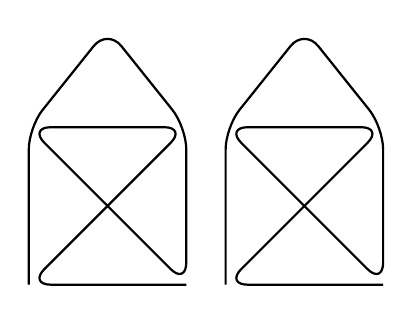
\begin{tikzpicture}
  \draw[thick,rounded corners=8pt]
    (0,0) -- (0,2) -- (1,3.25) -- (2,2) -- (2,0)
     -- (0,2) -- (2,2) -- (0,0) -- (2,0);
  \tcbpatcharcangular
  \draw[thick,rounded corners=8pt,xshift=2.5cm]
    (0,0) -- (0,2) -- (1,3.25) -- (2,2) -- (2,0)
     -- (0,2) -- (2,2) -- (0,0) -- (2,0);
\end{tikzpicture}
\end{dispExample*}

\end{docCommand}


\begin{docCommand}[doc new=2014-05-05]{tcbpatcharcround}{}
本宏还原 \refCom{tcbpatcharcangular}，即把
\refCom{tcbpatcharcangular} 的补丁替换回原有代码。
\end{docCommand}


\clearpage
\subsection{提取节点尺寸}
以下辅助宏由 \mylib{skins} 程序库定义。
它们可用于确定任意 \tikzname\ 节点的宽与高。
更确切地说，它们测定的是东西方向与南北方向的尺寸；
对于非矩形节点，这未必是最大尺寸。
注意，以下尺寸是连同边框线宽在内精确测量的。
若要据此绘制一个相同尺寸、带边框的新矩形或节点，
必须减去该边框宽度。

\begin{docCommand}[doc new=2014-09-19]{tcbsettowidthofnode}{\marg{register}\marg{node}}
  将所给 \meta{节点}的东西方向尺寸设置到 \TeX\ \meta{寄存器}中。
\end{docCommand}

\begin{docCommand}[doc new=2014-09-19]{tcbsetmacrotowidthofnode}{\marg{macro}\marg{node}}
  将 \meta{宏}定义为所给 \meta{节点}的东西方向尺寸。
\end{docCommand}

\begin{docCommand}[doc new=2014-09-19]{tcbsettoheightofnode}{\marg{register}\marg{node}}
  将所给 \meta{节点}的南北方向尺寸设置到 \TeX\ \meta{寄存器}中。
\end{docCommand}

\begin{docCommand}[doc new=2014-09-19]{tcbsetmacrotoheightofnode}{\marg{macro}\marg{node}}
  将 \meta{宏}定义为所给 \meta{节点}的南北方向尺寸。
\end{docCommand}

\begin{dispExample}
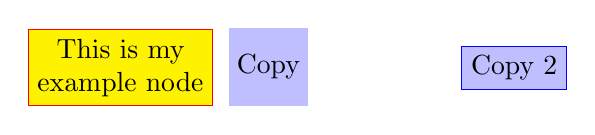
\begin{tikzpicture}
  \node[align=center,draw=red,fill=yellow] (A) {This is my\\example node};
  \tcbsetmacrotowidthofnode\mywidth{A}
  \tcbsetmacrotoheightofnode\myheight{A}
  \path[fill=blue!25!white]           %  rectangle without border
    ([xshift=2mm]A.south east)
    rectangle node{Copy} +(\mywidth,\myheight);
  \node[draw=blue,fill=blue!25!white, % standard border width 0.4pt
    minimum width=\mywidth-0.4pt,     % minus width of border
    minimum height=\myheight-0.4pt    % minus height of border
    ]
    at ([xshift=5cm]A) {Copy 2};
\end{tikzpicture}
\end{dispExample}


\subsection{超链接节点}
以下辅助宏由 \mylib{skins} 程序库定义。
\enlargethispage*{1cm}

\begin{docCommand}[doc new and updated={2016-02-03}{2023-02-28}]{tcbhypernode}{\marg{macro}\marg{node}}
%  Sets the east-to-west dimension of the given \meta{node}
%  to the \TeX\ \meta{register}.
  把 \refPkg{hyperref} 宏包 \cite{rahtz:hyperref} 中创建超链接的
  \meta{宏}应用到一个已有的 \tikzname\ \meta{节点}上。
  \refCom{tcbhypernode} 只能在 |tikzpicture| 环境内部使用。
  \meta{宏}的最后一个参数应省略，它本应代表要做成超链接的对象（文本）。
  例如，使用 |\hyperref[name]| 而非 |\hyperref[name]{text}|。

\begin{dispExample}
% \usepackage{hyperref}

\begin{tikzpicture}
  \node[align=center,draw=red,fill=red!5] (mybutton)
    {Click me to jump to Section~\ref*{sec:tikzimagefilling}};
  \tcbhypernode{\hyperref[sec:tikzimagefilling]}{mybutton}
\end{tikzpicture}
\end{dispExample}

\end{docCommand}

